\documentclass[a4paper,12pt]{article}
\usepackage[T1]{fontenc}
\usepackage{times}
\usepackage{amsmath}
\usepackage{amsfonts}
\usepackage{graphicx}
\usepackage{amssymb}
\usepackage{listings}
\usepackage{textcomp}
\usepackage{hyperref}
\usepackage{xcolor}

\title{Algorytmy numeryczne - projekt}
\author{Szymon Gosk, Damian Górski, Niuta Godlewska}

% commands

\newcommand{\id}{\noindent}
\newcommand{\el}[2]{\lambda_{(#1, #2)}}
\newcommand{\bl}[1]{\textbf{#1}}
\newcommand{\fa}[1]{\displaystyle\mathop{\forall}_{#1}}

\begin{document}

\maketitle

\newpage

\tableofcontents

\newpage

\section{Wstęp}

Niniejszy dokument stanowi dokumentacje wszystkich części projektu przedmiotu \textit{Algorytmy numeryczne}. Kolejne części projektu będą opisane w kolejnych sekcjach, a kolejne elementy poszczególnych częsci - w podsekcjach. \\

\id
Dokument ten jest również podsumowaniem pracy członków zespołu \textbf{1.1}, w którego skład wchodzą \textbf{Szymon Gosk}, \textbf{Damian Górski} i \textbf{Niuta Godlewska}. Członkowie zespołu wspólnie oświadczają, iż projekt był realizowany przez każdego z nich w równym stopniu zaangażowania. \\

\id
\bl{Kod wszystkich algorytmów} można znaleźć na repozytorium projektu:
\begin{center}
\textcolor{blue}{\href{https://github.com/Szymon-Gosk/szymon-gosk.github.io}{https://github.com/Szymon-Gosk/szymon-gosk.github.io}}
\end{center}
Kod umieszczony w tym dokumencie stałby się nieczytelny, tak więc - z uwagi na wygodę czytającego - zachęcamy do zapoznania się z programem na stronie zamieszczonej powyżej. \\

\id
Zaimplementowany projekt można znaleźć pod adresem: 
\begin{center}
\textcolor{blue}{\href{https://szymon-gosk.github.io/}{https://szymon-gosk.github.io/}}
\end{center}

\section{Interpolacja wielomianowa : Przyrost naturalny}

\subsection{Opis metod obliczeniowych}

\textbf{Zadanie}: Program, który oszacuje przyrost naturalnyna świecie w przyszłości. Węzły mają przedstawiać przyrost naturalny zmieniający się wczasie. \\

\id
Metoda numeryczna użyta w tym zadaniu to \textbf{metoda newtona}. Początkowo posiadamy zbiór $n+1$ danych: \\

$\{ (x_0, y_0), (x_1, y_1), ..., (x_n, y_n) \}$ \\

\id
Metoda polega na interpolacji danych w wielomian w postaci: \\

$P(x) = \sum\limits_{k=0}^{n}\left( b_k\prod\limits_{i=0}^{k-1}(x-x_i) \right )$ \\

\id
która pozwala oszacować wartości dla argumentów spoza zbioru danych. \\

\newpage

\id
Współczynniki $b_k$ można uzyskać korzystając z poniższego wzoru: \\

$b_k = \left( \frac{y_k \ - \ \sum\limits_{i=0}^{k-1}\left( b_i\prod\limits_{j=0}^{i-1}(x_k-x_j) \right)}{\prod\limits_{i = 0}^{k-1}(x_k - x_i)} \right)$ \\

\id
\bl{Przykład:} Dany jest następujący zbiór danych: \\

$\{ (2005, 6503), (2010, 6894), (2015, 7256) \}$ \\

\id
Zbiór współczynników dla tego zbioru to: \\

$b_0 = 6503$

$b_1 = 78.2$

$b_2 = -0.58$ \\

\id
przez co uzyskujemy wielomian w postaci: \\

$P(x) = 6503 + 78.2(x - 2005) - 0.58(x - 2005)(x - 2010)$ \\

\id
lub po przekształceniach: \\

$P(x) = -0.58x^2 + 2406.9 x - 2487717$ \\

\id
Korzystając z tego wielomianu można przybliżyć wynik dla dowolnej wartości $x$. Dla $x = 2020$ podstawiamy wartość: \\

$P(2020) = -0.58\cdot (2020)^2 + 2406.9\cdot 2020 - 2487717 = 7589$ \\

\id
Kolejnym krokiem jest metoda ogólna przekształcania wielomianu w postaci Newtona w postać ogólną: \\

$\sum\limits_{k=0}^{n}\left( b_k\prod\limits_{i=0}^{k-1}(x-x_i) \right ) = \sum\limits_{k=0}^{n}\left(a_kx^k\right)$ \\

\id
Obecnie, wielomian ma postać: \\

$b_0 + b_1(x-x_0) + b_2(x-x_0)(x-x_1) + ... + b_n(x-x_0)...(x-x_{n-1})$ \\

\id
Pierwszym krokiem będzie wymnożenie kolejnych iloczynów $(x-x_i)$ dla danego współczynnika $b_k$. W tym celu zdefiniujmy macierz $(n+1)\times (n+1)$: \\

$M=\begin{pmatrix}
\lambda_{(0,0)} & \lambda_{(0,1)} & \cdots & \lambda_{(0,j)} & \cdots & \lambda_{(0,n)}\\ 
\lambda_{(1,0)} & \lambda_{(1,1)} & \cdots & \lambda_{(1,j)} & \cdots & \lambda_{(1,n)}\\ 
\vdots & \vdots & & \vdots & & \vdots\\ 
\lambda_{(i,0)} & \lambda_{(i,1)} & \cdots & \lambda_{(i,j)} & \cdots & \lambda_{(i,n)}\\ 
\vdots & \vdots &  & \vdots &  & \vdots\\ 
\lambda_{(n,0)} & \lambda_{(n,1)} & \cdots & \lambda_{(n,j)} & \cdots & \lambda_{(n,n)}\\ 
\end{pmatrix}$ \\

\id
Zamysł elementów $\el{i}{j}$ jest następujący - zapiszmy wielomian w postaci opisanej wyżej: \\

$b_0 + b_1(x-x_0) + b_2(x-x_0)(x-x_1) + ... + b_n(x-x_0)...(x-x_{n-1}) = b_0\el{0}{0} + b_1(\el{1}{1}x+\el{0}{1}) + ... + b_n(\el{n}{n}x^n + \el{n-1}{1}x^{n-1} + ... + \el{0}{n}x^0)$ \\

\id
Innymi słowy, są to iloczyny kolejnych podwielomianów Newtona $\prod\limits_{i=0}^{k-1}(x-x_i)$. \\

\id
Konsekwencją tego jest fakt, iż: \\

$\fa{j<i}\el{i}{j} = 0$ \\

\id
co pozwala nam zapisać macierz $M$ jako: \\

$M = \begin{pmatrix}
\lambda_{(0,0)} & \el{0}{1} & \cdots & \el{0}{j} & \cdots & \el{0}{n}\\ 
0 & \lambda_{(1,1)} & \cdots & \el{1}{j} & \cdots & \el{1}{n} \\ 
\vdots & \vdots & & \vdots & & \vdots\\ 
0 & 0 & \cdots & \lambda_{(i,j)} & \cdots & \el{i}{n}\\ 
\vdots & \vdots &  & \vdots &  & \vdots\\ 
0 & 0 & \cdots & 0 & \cdots & \lambda_{(n,n)}\\ 
\end{pmatrix}$ \\

\id
Dodatkowo, warto zauważyć, że: \\

$\fa{i=j}\el{i}{j}=1$ \\

\newpage

\id
Do uzyskania postaci ogólnej wielomianu, należy dodać do siebie współczynniki $\lambda$ odpowiadające danym potęgom, pomnożone przez odpowiednie współczynniki $b$. Wykorzystamy do tego układ liniowy: \\

$\begin{pmatrix}
\lambda_{(0,0)} & \el{0}{1} & \cdots & \el{0}{j} & \cdots & \el{0}{n}\\ 
0 & \lambda_{(1,1)} & \cdots & \el{1}{j} & \cdots & \el{1}{n} \\ 
\vdots & \vdots & & \vdots & & \vdots\\ 
0 & 0 & \cdots & \lambda_{(i,j)} & \cdots & \el{i}{n}\\ 
\vdots & \vdots &  & \vdots &  & \vdots\\ 
0 & 0 & \cdots & 0 & \cdots & \lambda_{(n,n)}\\ 
\end{pmatrix}\cdot
\begin{pmatrix}
b_0 \\
b_1 \\
\vdots \\
b_i \\
\vdots \\
b_n
\end{pmatrix}
=
\begin{pmatrix}
a_0 \\
a_1 \\
\vdots \\
a_i \\
\vdots \\
a_n
\end{pmatrix}$ \\

\id
Rozwiązaniem tego układu dla poszczególnych $a_i$ jest: \\

$a_i = \sum\limits_{j=0}^{i}b_j\el{i}{j}$ \\

\id
Do wyznaczenia wzoru na współczynniki $\lambda$ posłużymy się kombinacjami. Niech zbiór $X$ będzie zbiorem współczynników $x_i$, tzn. $X = \{ x_0, x_1, ... , x_n\}$. Dodatkowo niech $X_i$ oznacza zbiór pierwszych $i$ współczynników zbioru \\ $X$: $X_i = \{x_1, x_2, ..., x_i \}$ \\

\id
Niech $C_j^i$ będzie zbiorem kombinacji o długości $j$ ze zbioru $X_i$: \\

$C_j^i = \binom{X_i}{j}$ \\

\id
Moc zbioru $C_j^i$ wyraża się przez $\vert C_j^i\vert = \binom{i}{j}$. Poniżej przedstawimy kilka kluczowych własności tego zbioru. \\

\id
Zbiór $C_j^i$ istnieje dla negatywnych wartości - przesłanka mówiąca za tym to fakt, że funkcja $\binom{i}{j} = \frac{\Gamma (i+1)}{\Gamma (j+1) \Gamma (i-y+1 )}$ jest zdefiniowana dla ujemnych wartości. \\

\id
Dodatkowo $\fa{ n\in \mathbb{N}}\fa{\alpha \in \mathbb{Z}^{-}}C^n_\alpha = \varnothing$ \ i \ $\vert C_\alpha^n\vert = 0$ \\

\id
Zdefiniowawszy powyższe rzeczy, lambdę możemy otrzymać ze wzoru: \\

$\el{i}{j} = (-1)^{(i+j)}\cdot \left( \sum\limits_{K \in C^j_{j-i}} \ \prod\limits_{x_k \in K} \left( x_k \right) \right)$ \\

\newpage

\id
co daje nam wzór ogólny na $a_i$: \\

$a_i = \sum\limits_{j=0}^{i} \left( (-1)^{(i+j)}\cdot b_j\left( \sum\limits_{K \in C^j_{j-i}} \ \prod\limits_{x_k \in K} \left( x_k \right) \right) \right)$ \\

\id
Teraz możemy zapisać wzór wielomianu w postaci ogólnej: \\

$P(x) = \sum\limits_{i=0}^{n} \left( x^i\sum\limits_{j=0}^{i} \left( (-1)^{(i+j)}\cdot b_j\left( \sum\limits_{K \in C^j_{j-i}} \ \prod\limits_{x_k \in K} \left( x_k \right) \right) \right) \right)$ \\

\id
\bl{Przykład:} Posłużymy się wielomian newtona z przykładu pierwszego: \\

$P(x)=6503+78.2\cdot(x-2005)-0.58\cdot(x-2005)(x-2010)$ \\

\id
Najpierw zapiszemy macierz współczynników lambda dla tego przykładu: \\

$
\begin{pmatrix}
\el{0}{0} & \el{0}{1} & \el{0}{2} \\
0 & \el{1}{1} & \el{1}{2} \\
0 & 0 & \el{2}{2} &\\
\end{pmatrix}
$ \\

\id
Następnie, posługując się wcześniej zdefiniowanym zbiorem $C_j^i$, obliczamy: \\

$C^0_0 = C^1_0 = C^2_0 = \{ \varnothing \}$ \\

$C^1_1 = \{ \{x_0\} \}$ \\

$C^2_2 = \{ \{x_0, x_1 \} \}$ \\

$C^2_1 = \{ \{x_0\}, \{ x_1 \} \}$ \\

\id
Co pozwala obliczyć nam współczynniki lambda: \\

$\el{0}{0} = \el{2}{2} = \el{1}{1} = \sum\limits_{K \in C^1_{0}} \ \prod\limits_{x_k \in K} \left( x_k \right) = \sum\limits_{K \in \{ \varnothing \}} \ \prod\limits_{x_k \in K} \left( x_k \right) = \prod\limits_{x_k \in \varnothing} \left( x_k \right) = 1$ \\


$\el{0}{1} = -\sum\limits_{K \in C^1_{1}} \ \prod\limits_{x_k \in K} \left( x_k \right) =  -\sum\limits_{K \in \{ \{x_0\} \}} \ \prod\limits_{x_k \in K} \left( x_k \right) = -\prod\limits_{x_k \in \{x_0\}}x_k = -x_0 = -2005$ \\


$\el{0}{2} = \sum\limits_{K \in C^2_{2}} \ \prod\limits_{x_k \in K} \left( x_k \right) =  \sum\limits_{K \in \{ \{x_0, x_1\} \}} \ \prod\limits_{x_k \in K} \left( x_k \right) = \prod\limits_{x_k \in \{x_0, x_1\}}x_k = x_0x_1 = 4030050$ \\


$\el{1}{2} = -\sum\limits_{K \in C^3_{2}} \ \prod\limits_{x_k \in K} \left( x_k \right) = -\sum\limits_{K \in \{ \{x_0\}, \{x_1\} \}} \ \prod\limits_{x_k \in K} \left( x_k \right) = -\left( \prod\limits_{x_k \in \{x_0\}}x_k + \prod\limits_{x_k \in \{x_1\}}x_k \right) = -(x_0 + x_1) = -4015$ \\



\id
Zapisujemy równanie liniowe z wyliczonymi współczynnikami $\lambda$: \\

$
\begin{pmatrix}
1 & -2005 & 4030050 \\
0 & 1 & -4015 \\
0 & 0 & 1 &\\
\end{pmatrix}
\begin{pmatrix}
6503 \\
78.2 \\
-0.58 \\
\end{pmatrix}
=
\begin{pmatrix}
a_0 \\
a_1 \\
a_2 \\
\end{pmatrix}
$ \\

\id
Z czego otrzymujemy: \\

$a_0 = 6503 - 2005\cdot 78.2 - 0.58\cdot 4030050 = -2487717$ \\

$a_1 = 78.2 + 4015\cdot 0.58 = 2406.9$ \\

$a_2 = -0.58$ \\

\id
A następnie podstawiając otrzymujemy poprawny wielomian w postaci ogólnej: \\

$P(x) = -0.58x^2 + 2406.9x - 2487717$

\subsection{Opis implementacji algorytmu}

\id
Implementacja składowych całościowego algorytmu jest prosta z uwagi na matematyczny zapis obliczeń. Każda suma lub iloczyn, jest równaważny pętli w programie. \\

\id
Pierwszym elementem algorytmu jest wyliczenie współczynników $b$. Program oblicza je zgodnie z podanym wzorem, a do liczenia każdej sumy lub iloczynu wykorzystuje pętlę. \\


\id
Po obliczeniu współczynników $b$, program tworzy \textit{String}, w którym zawiera dane współczynniki, wartości $x_i$ i zwraca \textit{String} zawierający postać Newtona wielomianu konkatenując współczynniki z nazwiasami i wartościami $x_i$. \\

\id
Korzystając z powstałego wielomianu program pobiera argument wpisany przez użytkownika i wylicza wartośc wielomianu dla tego argumentu. \\

\id
Z racji na skomplikowanie algorytmu przekształcania postaci Newtona w postać ogólną, implementacja została pominięta, a metoda zostawiona w dokumencie jako ciekawostka.

\subsection{Struktury danych i struktura programu}

\id
Program wykorzystuje proste listy, jeden z podstawowych typów danych w języku \textit{Javascript}. \\

\id
Dodatkowo przeprowadzane są operacje na liczbach - \textit{float} - a także, w celu wyświetlania rezultatów, na danych typu \textit{String}. \\

\id
Struktura skryptu obliczeniowego odpowiada warstwie teoretycznej implementacji - tj. kolejnośc wykowywanych zadań w jednym skrypcie jest taka sama jak w sekcji \textbf{2.1} oraz \textbf{2.2}. \\

\id
Wykorzystane zostały biblioteki KaTeX - do tworzenia tekstu matematycznego - i JsXGraph do tworzenia wykresów.

\subsection{Program}

\id
Poniżej zostały zaprezentowane przykłady działania programu dla różnych przypadków: \\

\begin{center}
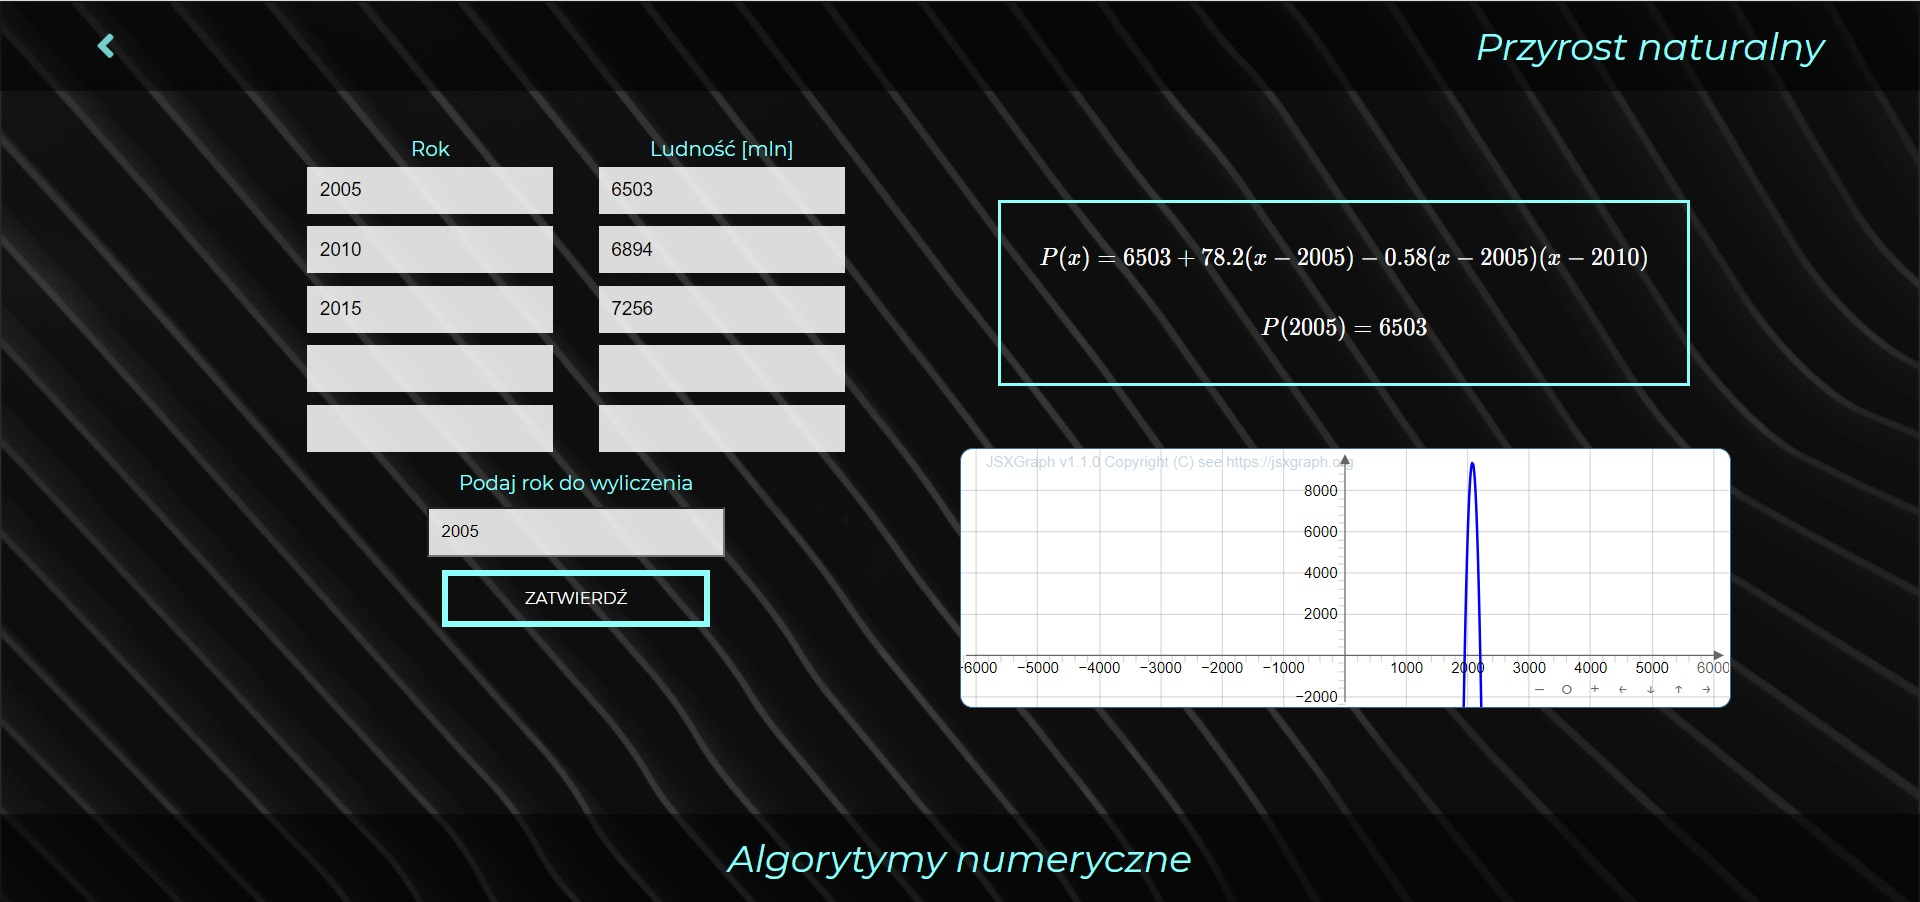
\includegraphics[width=1\textwidth]{proj1sc1.jpg} \\
\end{center} 

\begin{center}
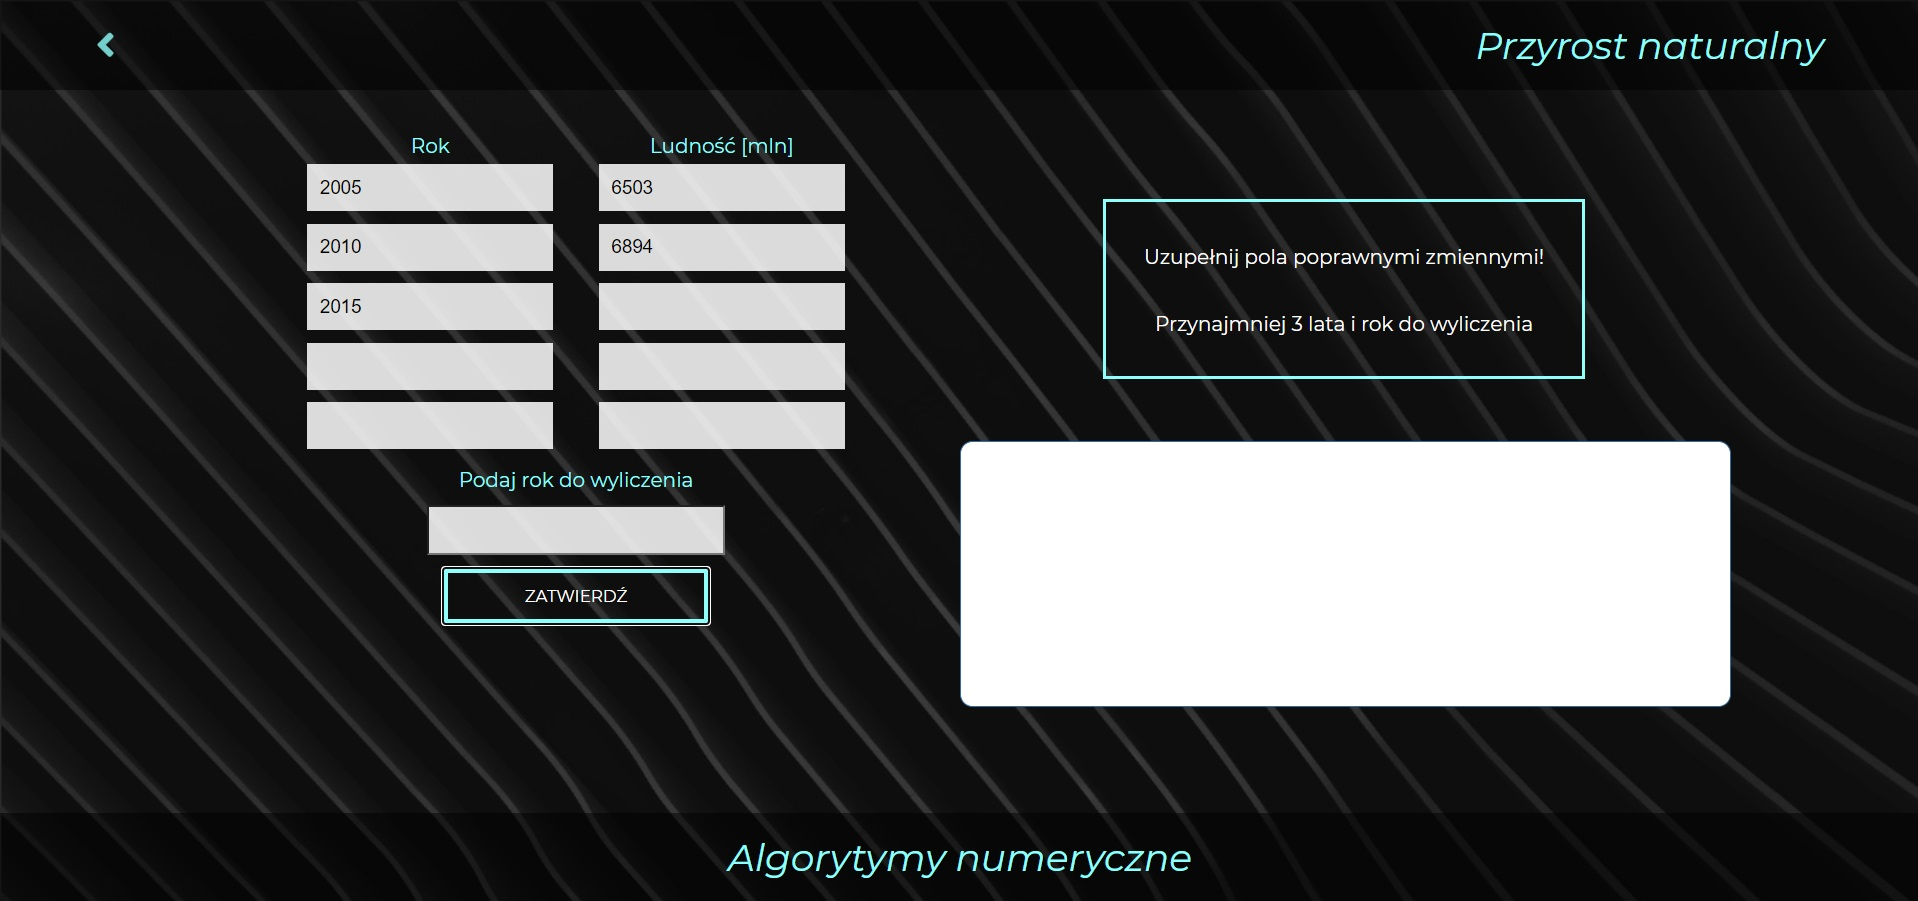
\includegraphics[width=1\textwidth]{proj1sc2.jpg} \\
\end{center} 

\begin{center}
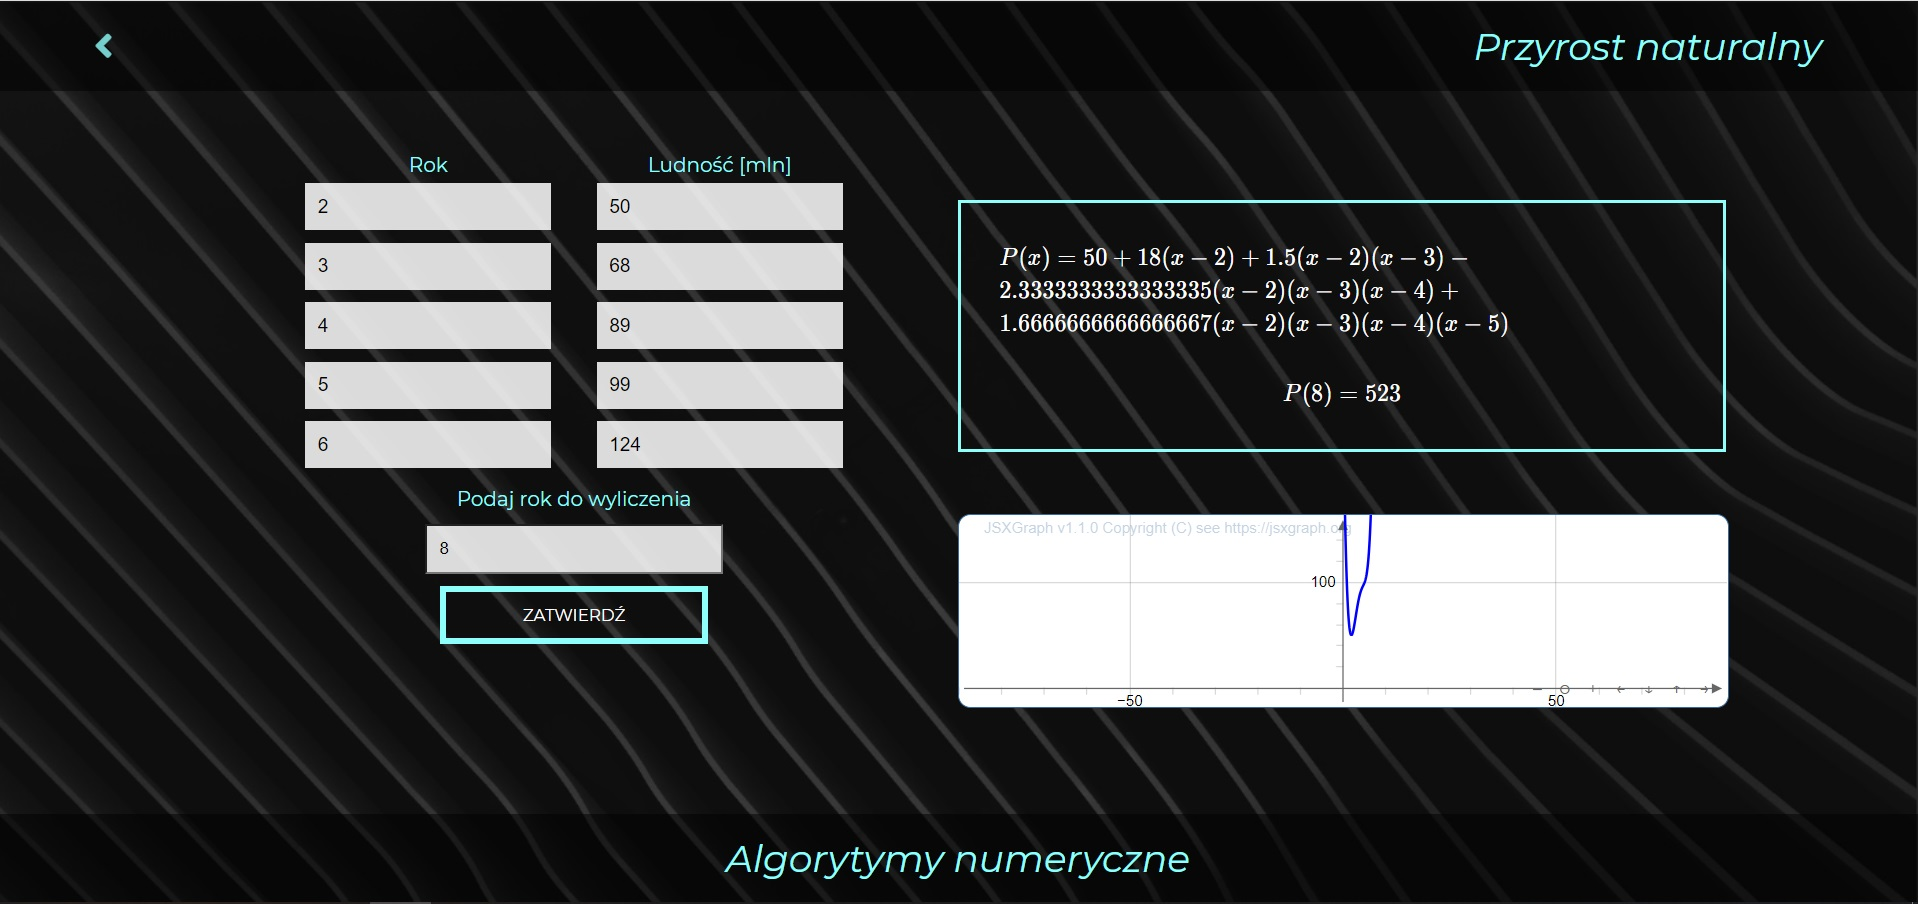
\includegraphics[width=1\textwidth]{proj1sc3.jpg} \\
\end{center} 

\begin{center}
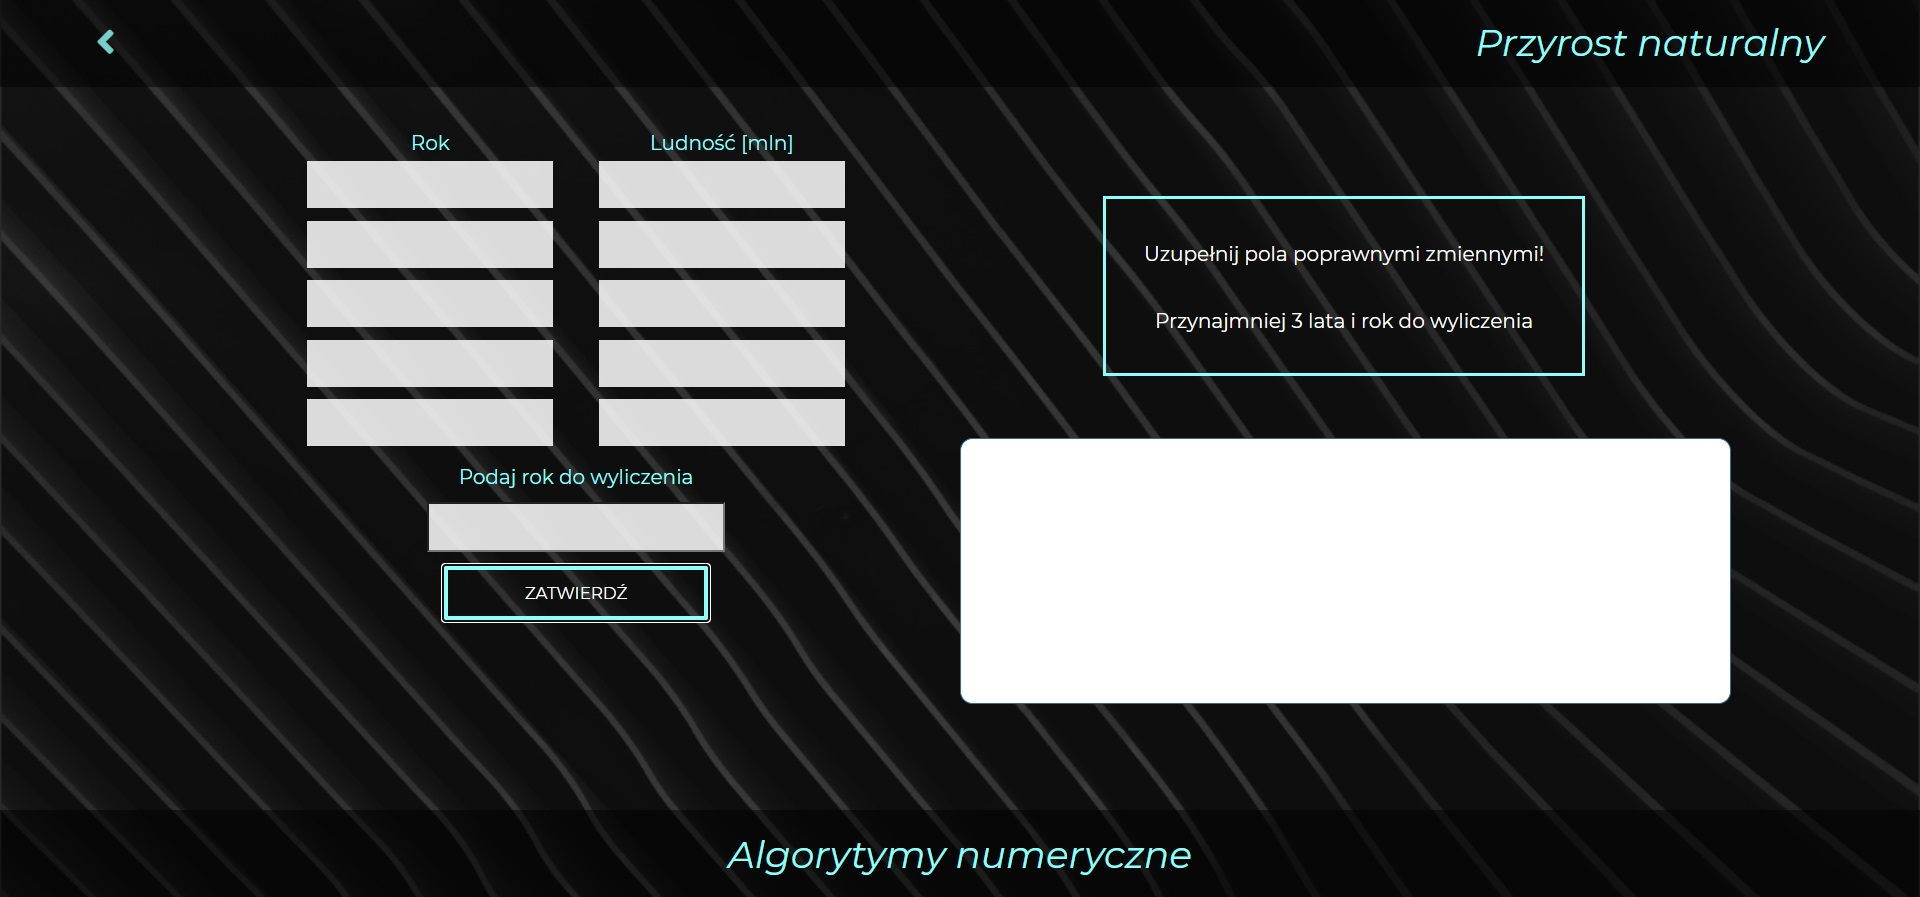
\includegraphics[width=1\textwidth]{proj1sc4.jpg} \\
\end{center} 

\subsection{IO (wejście-wyjście)}

\id
Wejściowe dane w programie są podawane w kontenerach typu \textit{input}: \\

\begin{lstlisting}
<input type="number" (...) class="input-v">
\end{lstlisting} 

\id
I pobierane przez program w skrypcie \textit{JQuery} po naciśnięciu przycisku. Akceptowane są tylko wartości liczbowe, które mimo wszystko przechodzą do programu jako \textit{String} - skrypt zamienia je po ich wprowadzeniu na wartości liczbowe. \\

\id
Program sprawdza, czy podano poprawne dane, tj. czy liczba podanych lat i wartości zgadza się, czy nie pozostawiono jednego z pól pustego, czy podano wartość do wyliczenia. Jeśli znaleziony zostanie błąd, program wyświetli odpowiedni komunikat w kontenerze. \\

\id
Dane wyjściowe programu to wartości $String$ zawierające wzór wielomianu - wzór użyty do wyświetlenia wielomianu jest renderowany przez bibliotekę $KaTeX$ na podstawie "brzydkiego", wyliczonego wzoru. Program na podstawie "brzydkiego" wzoru generuje również wykres funkcji przez bibliotekę JsXGraph. Dodatkowo pojawia się wyliczona wartość aproksymacji dla podanego roku. 

\section{Projekt nr 2}

\section{Projekt nr 3}


\end{document}
